\documentclass{article}
\usepackage{cancel}
\usepackage{gensymb}
\usepackage{tikz}
\usetikzlibrary{angles,quotes}
\usetikzlibrary{arrows.meta,calc}


\title{Astro HW 2}
\author{Pierson Lipschultz}

\begin{document}
\maketitle
\setcounter{section}{1}
\section{}
\subsection{}
\subsubsection{a}

\[d_{lim} = \frac{1au}{\tan(\frac{1}{20})} = 1145au \]
\[ d_{proxC} \approx \frac{1au}{\tan(\frac{1}{360})} = 20626au \]
\[d_{proxC} > d_{lim}\]

\subsubsection{b}

\[d = \frac{1au}{\tan(.1 \times 10^{-3}/3600)} = 2062648062au\]
\[d_{pc} = \frac{2062648062au}{206266.372} \approx 9999.92pc \]

\subsection{}

\subsubsection{a}
\[\theta_a = \omega_{a} \Delta t + \beta a  \]
\[\theta_b = \omega_{b} \Delta t + \beta b  \]
\subsubsection{b}

\[ \omega_a\Delta t + \beta_a - \omega_b\Delta t - \beta_b = 2\pi\]
\[ \omega_a\Delta t + \cancel{\beta_a} - \omega_b\Delta t - \cancel{\beta_b} = 2\pi\]
\[ \omega_a\Delta t  - \omega_b\Delta t = 2\pi\]
\[ \omega_a(t_2-t_1)  - \omega_b(t_2-t_1) = 2\pi\]
\[ \frac{2\pi}{p_a}(t_2-t_1)  - \frac{2\pi}{p_b}(t_2-t_1) = 2\pi\]
\[ \frac{1}{p_a}  - \frac{1}{p_b} = \frac{1}{p_{syn}}\]


\subsubsection{c}


\[ \frac{1}{p_p}  =  \frac{1}{p_E} + \frac{1}{p_{syn}}\]

\subsubsection{d}

\[  - \frac{1}{p_E} = \frac{1}{p_{syn}} -  \frac{1}{p_p}\]
\[  \frac{1}{p_E} =  \frac{1}{p_p} - \frac{1}{p_{syn}}\]

\subsubsection{e}

\[  \frac{1}{p_E} =  \frac{1}{p_p}- \frac{1}{p_{syn}}\]
\[\frac{1}{p_{syn}} = \frac{1}{p_p} - \frac{1}{p_E}\]
\[\frac{1}{p_{syn}} = \lim_{P_p \rightarrow \infty} \frac{1}{p_p} - \frac{1}{p_E} \rightarrow \frac{1}{p_{syn}} = - \frac{1}{p_E}\]
\begin{center}
    if the superior planet has a very long orbital period, then the time of opposition will approach the period of the inferior planet.
\end{center}

\subsubsection{f}

\[\frac{1}{p_{syn}} =  \frac{1}{p_E} - \lim_{P_p \rightarrow p_E}\frac{1}{p_p}\rightarrow \frac{1}{p_{syn}} = 0\]


\subsubsection{g}

\[\frac{1}{P_{syn}} = \frac{1}{365.256} - \frac{1}{1.881*365.256}\]
\[p_{syn} = 779.8 days\]

\[\frac{1}{P_{syn}} = \frac{1}{365.256} - \frac{1}{164.79*365.256}\]
\[p_{syn} = 367.23 days\]

Yes, this makes sense. As we found from subsection e, if a superior planet has a much greater orbit period then the inferior (like Neptune), the period approaches that of the inferior.

From part F we found that the closer two planets period are to one another, the greater $P_{syn}$ becomes.

In this problem we see that with Neptune, a planet with much greater orbital period then Earth, $P_{syn}$ is close to $P_{earth}$, whereas with Mars, $P_{syn}$ has grown longer.

\subsection{}
\subsubsection{a}


\begin{center}
  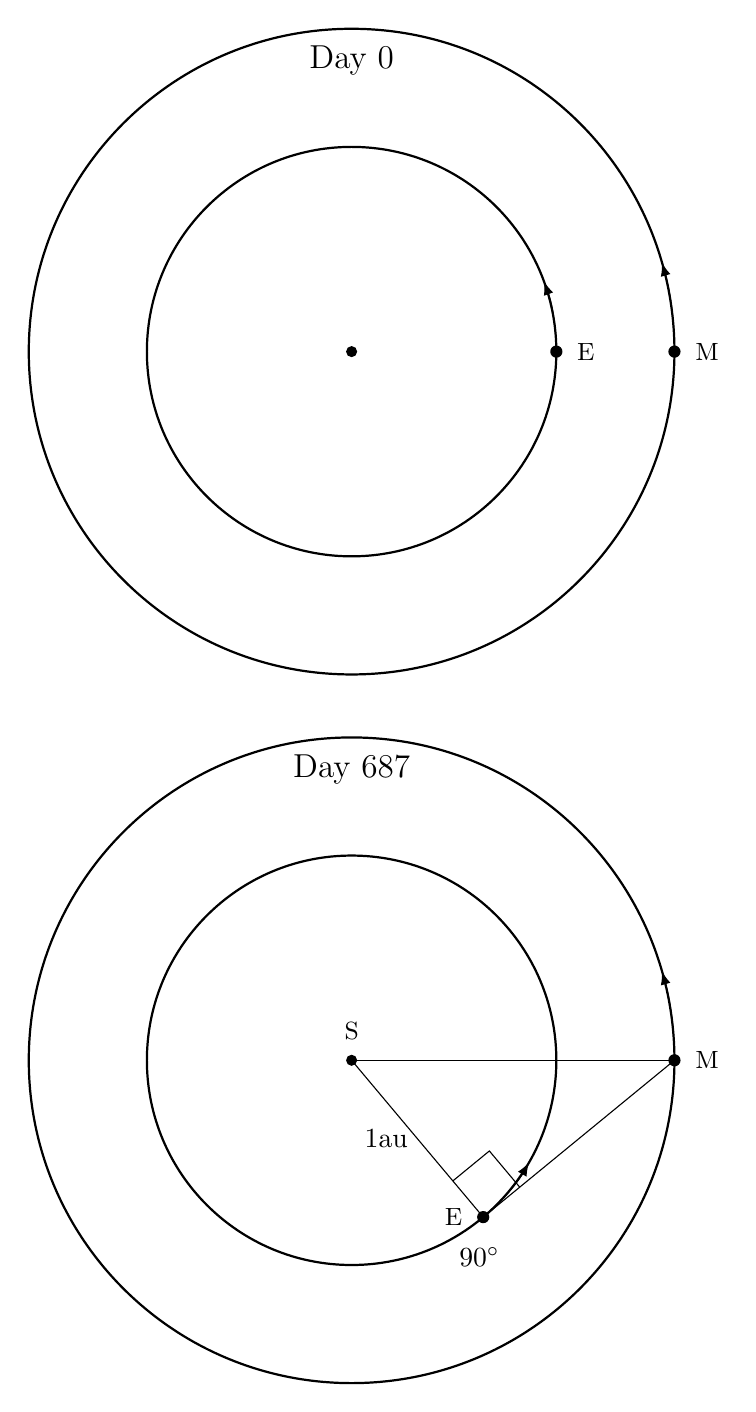
\begin{tikzpicture}[>=Latex]
  
  % --------- knobs you can tweak ----------
  \def\RE{2.6}   % Earth orbit radius
  \def\RM{4.1}   % Mars orbit radius
  
  % Angles after 687 days
  \def\angE{310} % Earth angle (approx)
  \def\angM{360*687/687} % ~360 deg, one full orbit
  % ----------------------------------------
  
  % ============== Panel: Day 0 =================
  \begin{scope}[shift={(0,0)}]
    \node[font=\large] at (0,3.7) {Day 0};
  
    % Sun
    \fill (0,0) circle (2pt);
  
    % Orbits
    \draw[thick] (0,0) circle (\RE);
    \draw[thick] (0,0) circle (\RM);
  
    % Positions
    \coordinate (E0) at (\RE,0);
    \coordinate (M0) at (\RM,0);
  
    \fill (E0) circle (2.2pt);
    \fill (M0) circle (2.2pt);
  
    % Labels outside orbit
    \node[right=4pt] at (E0) {\small E};
    \node[right=4pt] at (M0) {\small M};
  
    % Motion arrows
    \draw[->] (\RE,0) arc (0:20:\RE);
    \draw[->] (\RM,0) arc (0:16:\RM);
  \end{scope}
  
  % ============== Panel: Day 687 =================
  \begin{scope}[shift={(0,-9)}]
    \node[font=\large] at (0,3.7) {Day 687};
  
    % Sun
    \fill (0,0) circle (2pt);
  
    % Orbits
    \draw[thick] (0,0) circle (\RE);
    \draw[thick] (0,0) circle (\RM);
  
    % Positions after 687 days
    \coordinate (E1) at (\angE:\RE);
    \coordinate (M1) at (0:\RM); % Mars ~back to start after 1 orbit
  
    \fill (E1) circle (2.2pt);
    \fill (M1) circle (2.2pt);
  
    % Labels outside orbit
    \node[left=4pt] at (E1) {\small E};
    \node[right=4pt] at (M1) {\small M};
    \node[above=4pt] at (0,0) {\small S};
  
    % Motion arrows
    \draw[->] (\angE:\RE) arc (\angE:\angE+20:\RE);
    \draw[->] (0:\RM) arc (0:16:\RM);

  \coordinate (S) at (0,0);   % Sun
  \coordinate (E) at (E1);   % Earth
  \coordinate (M) at (M1);   % Mars

  % Triangle
  \draw (E) -- (M);
  \draw (E) -- (S) node[midway, left]{1au};
  \draw (S) -- (M);

  % Mark right angle at E (between S--E--M)
  \pic[draw,angle radius=6mm,"$90^\circ$"] {right angle = S--E--M};

  \end{scope}
  
  \end{tikzpicture}
\end{center}


\subsubsection{b}

\[\frac{360}{365.25} = .9856 deg/day\]
\[687* .9856 = 677.125 \]
\[677.125 - 360 = 317.125\]
\[360 - 317.125 = 42.874 = \theta_{\angle MSE}\]
\[180 - 42.874 - 90 = 47.125 =  \theta_{\angle SME}\]

\subsubsection{c}
\[SM = D_{mars}\]
\[cos(42.874) = \frac{1}{SM}\]
\[SM = \frac{1}{\cos 42.874}\]
\[SM = 1.36\]
\[D_{mars} = 1.36 AU\]

\subsubsection{d}

\[\arctan(\frac{3390}{5.236 \times 10^6}) \times 3600 \]
\[ 13.35 \times 2 \]
\[\theta_{arcsec}\approx 26.708\]


\subsection{}

\[c = \frac{d}{dx} \frac{a}{cos\theta}\]
\[c(\theta) = a\frac{sin\theta}{cos\theta^2} \equiv a\frac{tan\theta}{cos\theta}\]

\begin{center}
\begin{tabular}{|c|c|}
\hline
 $\theta$ & $c(\theta)$ \\
 \hline
 87 & $\approx$ $a364.58$ \\
 88 & $\approx$ $a820.5$ \\
 89 & $\approx$ $a3282.63$ \\
 89.8 & $\approx$ $a82069.992$ \\
\hline
\end{tabular}
\end{center}
\end{document}